Ein weiterer Teil der Aufgabe befasste sich mit dem Greifen der Tasse. Dafür steht der Greifer Schunk PG70 zur Verfügung, sowie ein 3D-Drucker zur Erstellung von Fingern. Zu Beginn wurden zwei Griffvarianten in Betracht gezogen: 1) Seitliches Greifen und 2) Greifen von oben. Während seitliches Greifen natürlicher erscheint, erwies sich die Planung für einen Griff der Tasse von oben als einfacher. Um keine Variante vorzeitig auszuschließen, wurde ein Fingermodell mit zwei möglichen Griffflächen erstellt, eine Fläche am Ende des Fingers, sowie eine Ausbuchtung am Schaft des Fingers. Die Fläche am Endes des Fingers führte zu genau zwei Kontaktpunkten zwischen der Tasse und dem Endeffektor. Die Tasse wurde sehr instabil gehalten und neigte zu Schaukeln bei schnelleren Bewegungen. Desweiteren reichte die Reibung zwischen Kunststoff und Ton nicht für einen festen Griff aus.

Aus diesem Grund wurde die Anzahl der Kontaktpunkte durch eine eckige Ausbuchtung von zwei auf vier verdoppelt. Bei ersten Tests mit der eigentlichen Hardware wurde ein weiteres Problem erkannt: Der Gesamthub des Greifers ist geringer als der durchschnittliche Durchmesser der Tasse. Daher konnte zuerst nur eine von zwei Tassen gegriffen werden, außerdem beschränkte sich die Pufferzone auf weniger als 1cm pro Fingerbacke. Die ersten Ergebnisse aus der Bilderkennung legte eine deutliche Verbreitung der Griffbreite nahe, um Ungenauigkeiten bei der Approximation der Tasse auszugleichen.

Die folgende Generation an Fingern vergrößerte die Griffbreite um 4cm durch \glqq Nach-hinten\grqq -Lagerung jeder Backe. Zusätzlich wurde der Schaft verlängert und erhielt eine ähnliche kantige Ausbuchtung, wie bereits das Ende des Fingers. Diese Änderung vergrößerte den Arbeitsbereich des Roboters, den Sicherheitsabstand zum Tisch und die Kontaktfläche der Tasse am Schaft des Fingers.

Bei einem weiteren Versuch wurde durch einen Konfigurationsfehler zu tief unter die Kante der Tasse eingetaucht, was in letzter Konsequenz zum Brechen eines Fingers führte. Um dieses Problem bei einer weiteren Iteration kategorisch auszuschließen, wurde die Verschiebung des Schaftes an den Montagebereich gelegt, eine abfallende Kante in Richtung Ende des Fingers konstruiert und die Gesamtlänge von 12cm auf 11cm reduziert. Außerdem wurde die Druckrichtung von Horizontal auf Vertikal verändert, um die Stabilität zu erhöhen.

Zusätzlich wurden zwei Varianten für eine bessere Reibung getestet: 1) Arbeitshandschuh und 2) Haushaltsgummi. Aus dem Handschuh wurden zwei Finger entfernt und mit doppelseitigem Klebeband auf dem gedruckten Finger befestigt. Der Grip zwischen Finger und Tasse erhöht sich, jedoch ist die hinzugefügte Schicht dünn, weshalb der Finger sich bei erhöhtem Druck verbiegt. Zur Vermeidung wird eine dickere Schicht zwischen Finger und Tasse benötigt. Haushaltsgummis in einem X-Muster erwiesen sich als besser geeignet, da sie mehr Reibung und eine dickere Schicht bieten.

\begin{figure}
    \centering
    \begin{minipage}{0.45\textwidth}
        \centering
        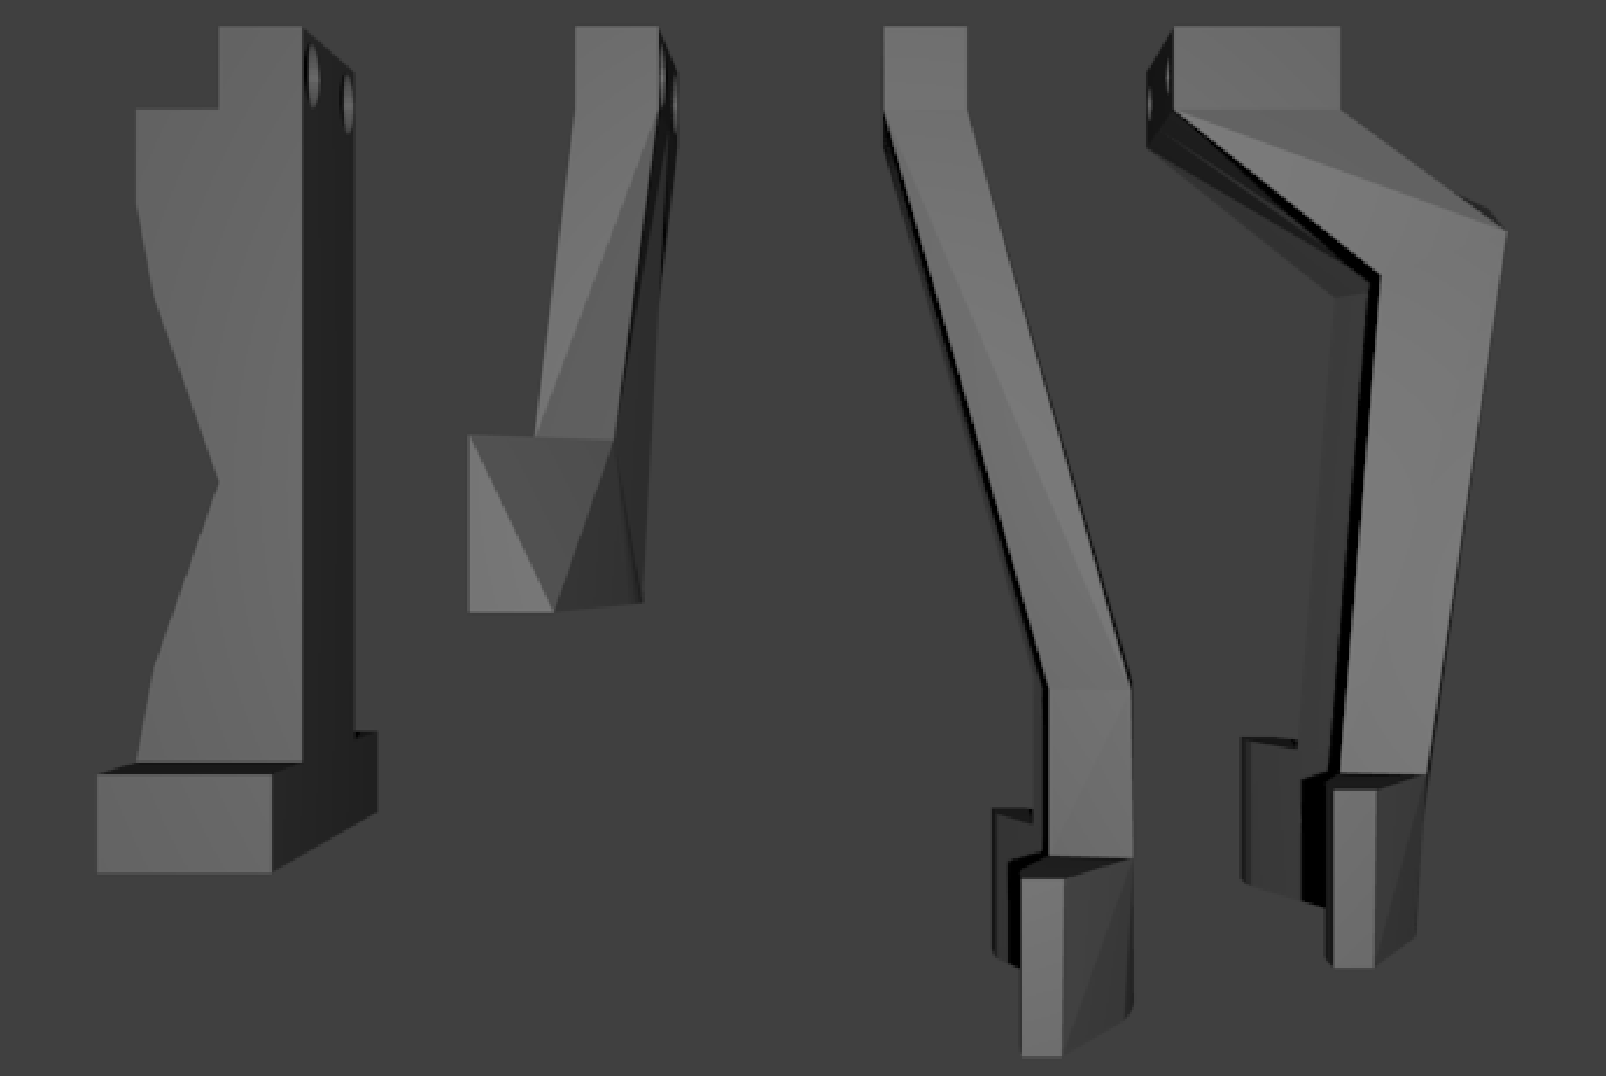
\includegraphics[width=0.9\textwidth]{images/finger_evolution.png} % first figure itself
        \caption{Evolution des Fingers}
    \end{minipage}\hfill
    \begin{minipage}{0.45\textwidth}
        \centering
        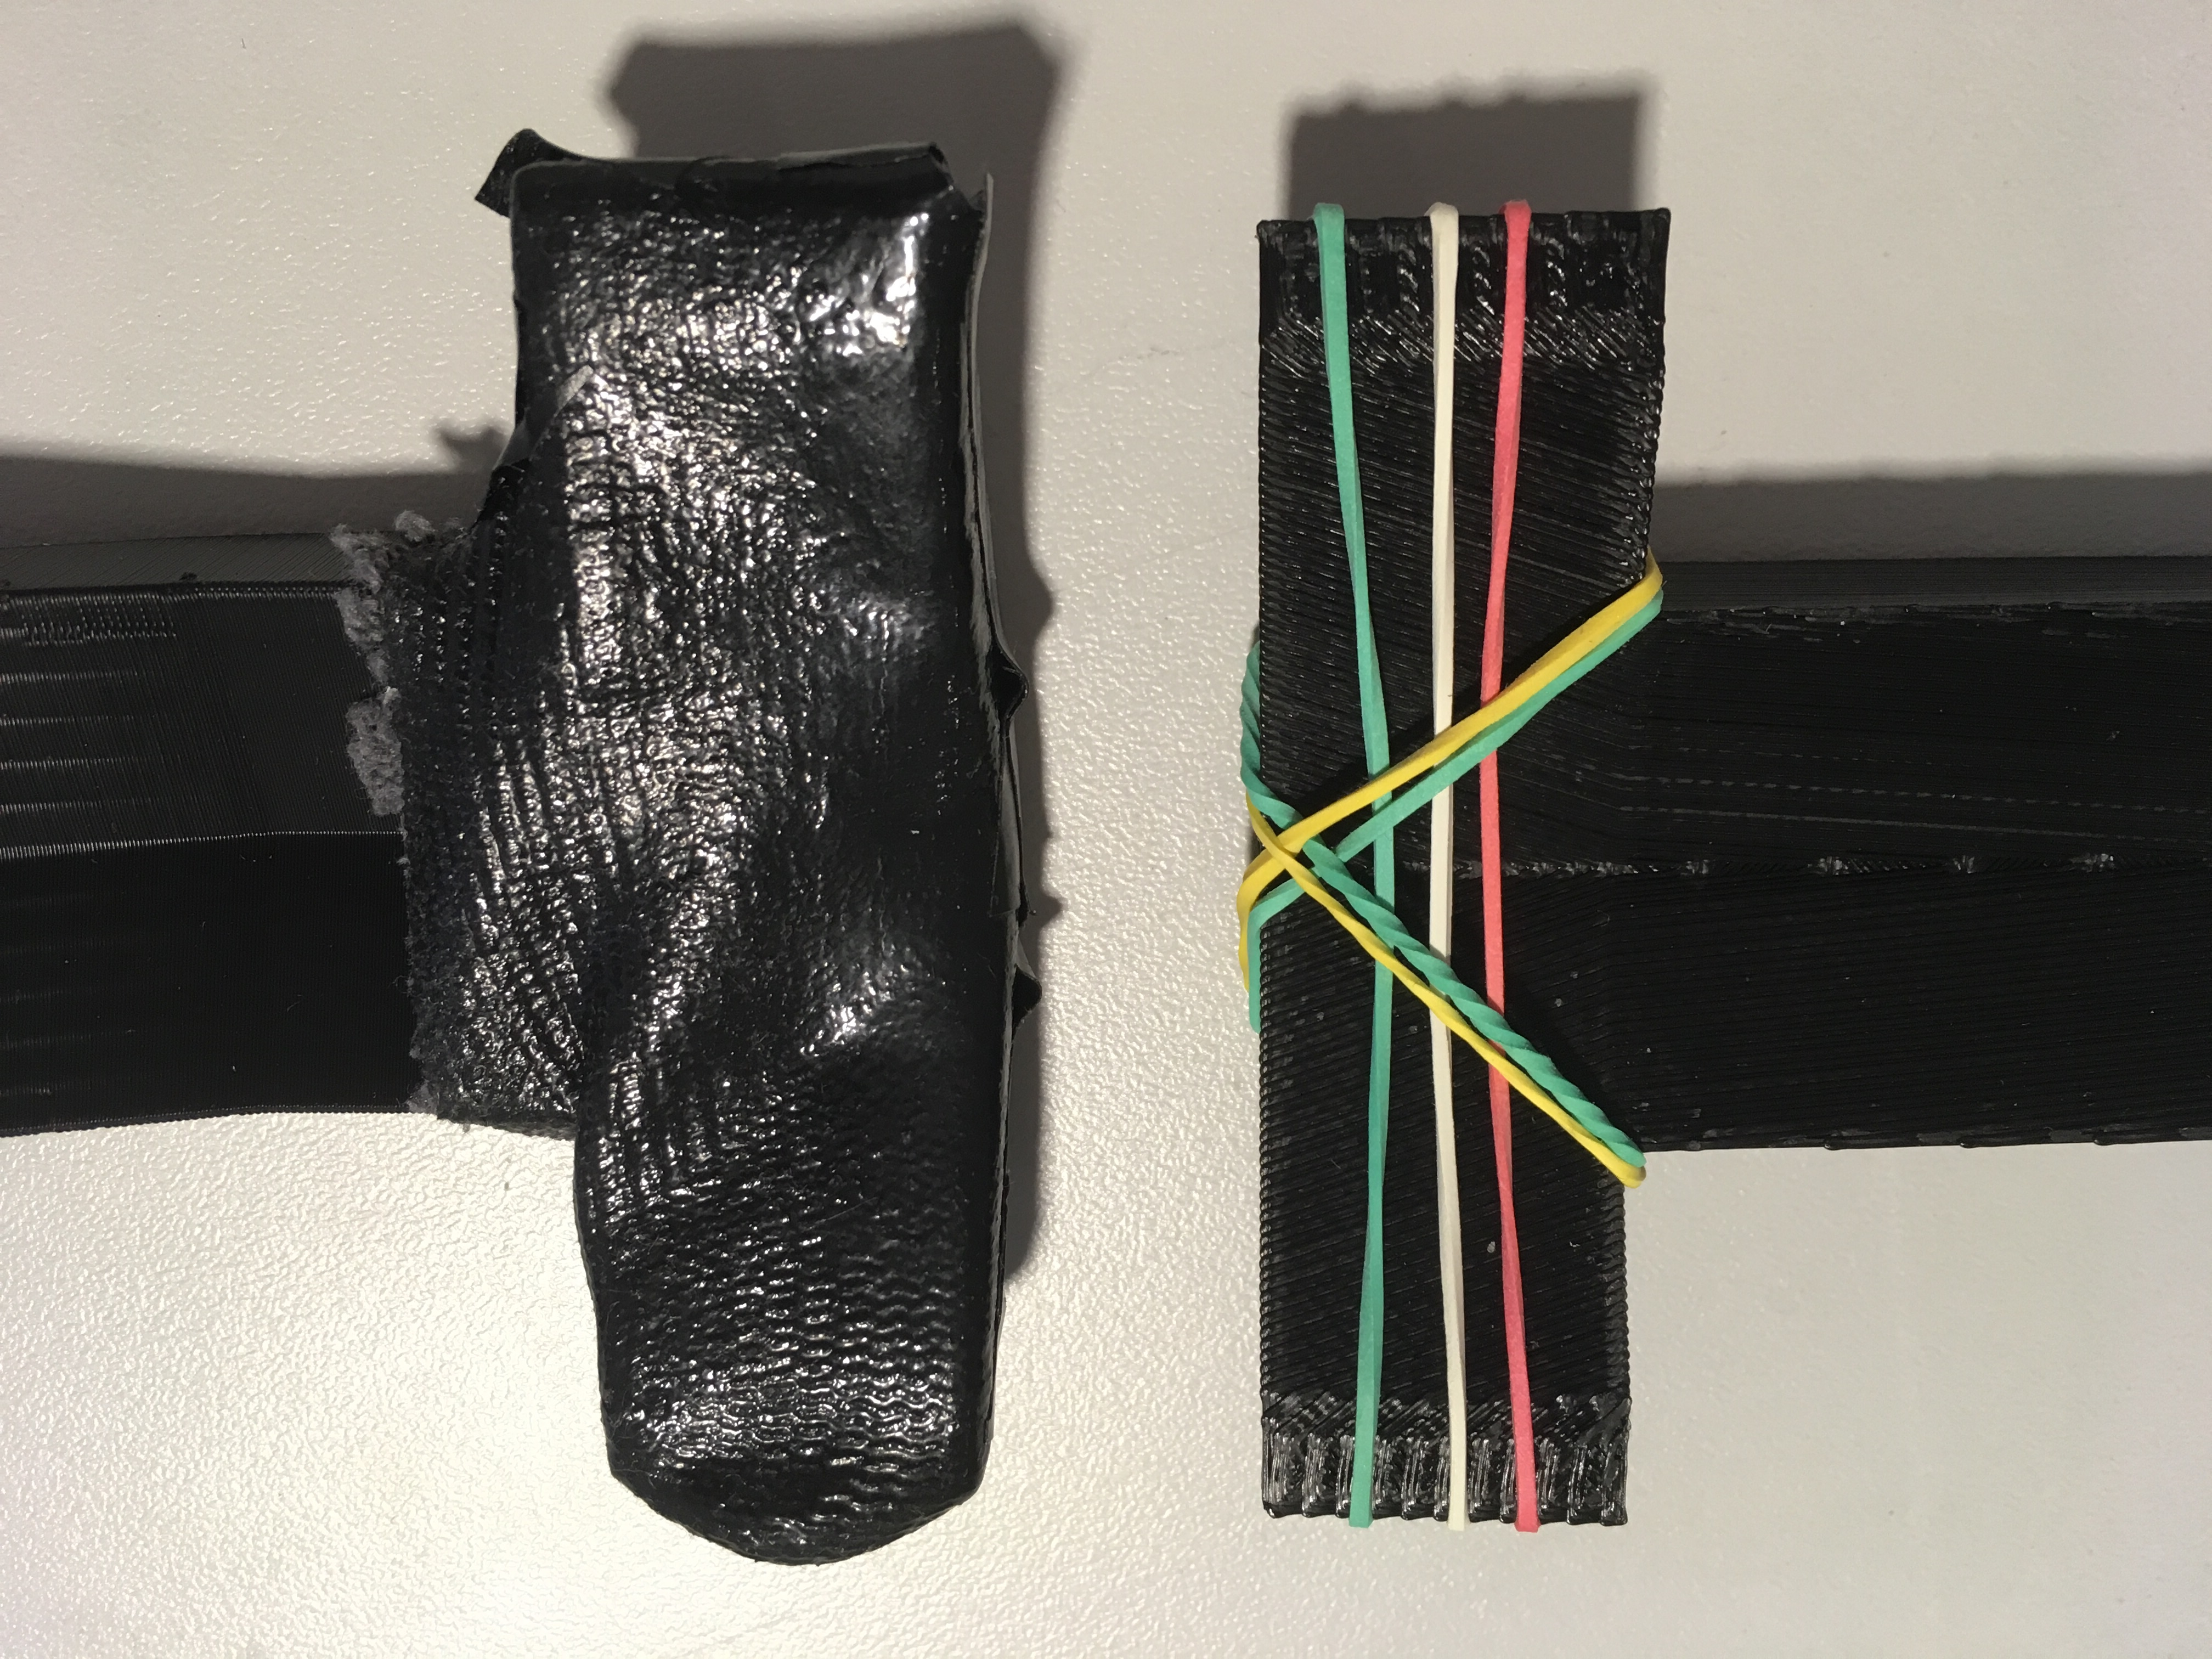
\includegraphics[width=0.9\textwidth]{images/finger_tip.JPG} % second figure itself
        \caption{Erhöhter Grip}
    \end{minipage}
\end{figure}

Abhängig von der Tasse wurden verschiedene Konstanten für die Breite der Finger empirisch getestet. Zur Vereinfachung gehen wir nun von genau einem Tassenmodell mit einer festen Breite aus. Anfangs wurde mit einem Fingerabstand von 9mm gegriffen, jedoch lässt sich dieser Wert zugunsten der Grifffestigkeit deutlich verkleinern. Es zeigte sich, dass bereits ein Abstand von 8mm ausreicht.

Nebenläufig zur Evolution der Finger wurde ein ROS Paket mit dem Namen \glqq cup\_ gripper\grqq  erstellt. Die erste Variante beinhaltete zwei Services: GrabCup und ReleaseCup. GrabCup akzeptierte als Parameter cup\textunderscore diameter in Meter und gab, wie auch ReleaseCup, ein boolean success zurück. Es stellte sich heraus, dass Actions besser geeignet sind, da sie längere Operationen abbilden und Feedback geben können. Aus diesem Grund wurden die Services in Actions umgeschrieben.
